
\hypertarget{contexte-general}{%
\section{Contexte général}\label{contexte-guxe9nuxe9ral}}
\subsection{Qu'est ce que le sudoku}

Le sudoku est un jeu représenté par une grille de 81 case découpé en 9 lignes et 9 colonnes et 9 sous-grilles 3 par 3.
Le but du jeu est de remplir chaque ligne avec 9 chiffre allant de 1 à 9 en faisant en sorte qu'il n'y ai pas le même chiffre plusieurs fois sur la même ligne colonne ou dans la même sous grille.

\begin{figure}[!h]
\centering
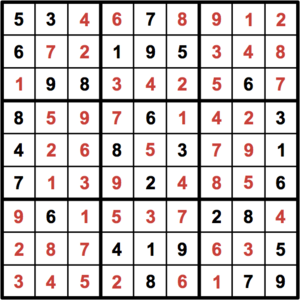
\includegraphics[width=10cm]{./images/Sudoku_Exemple.png}\label{Sudoku}
\caption{Exemple de Sudoku complet.}
\end{figure}

\hypertarget{Contexte du problème}{%
\section{Contexte du problème}\label{Contexte_du_probleme}}

La résolution de sudoku est un sujet ou plusieurs solutions existent et où c'est dans la complexité\footnote{le nombre d'action réalisé durant la résolution} des différentes solution que réside la difficulté la résolution. Nous pouvons aussi rendre compte de résolution de sudoku avec des règles spécifiques.
tel que:

\begin{figure}[!h]
\centering
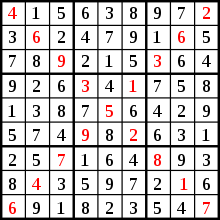
\includegraphics[width=10cm]{./images/Sudoku_Special.png}\label{Sudoku_Special}
\caption{Exemple de Sudoku où on applique la règle de l'unicité des chiffres sur les diagonnales.}
\end{figure}
